\section{问题描述}
本题需要我们根据表\ref{tab:data}给出的1790—1880年美国人口数据，分别利用Malthusian模型和Logistic模型进行参数估计，并预测1890—1980年的人口，最后比较两种模型的预测精度。
依据题目要求，我们将采用田心教授\cite{tianxin}书中第5章（模型辨识与参数估计）中的方法解决问题。
其中，Logistic模型需要采用等时间间隔三点法的方式估算参数$r$和$\bar{N}$，确定参数后再进一步估计美国1890-1980年的人口数据。
\par
题目给出的1790—1880年的美国人口数据如下表所示：
\begin{table}[h]
\centering
\caption{1790—1880年美国人口数据（单位：千人）}
\label{tab:data}
\begin{tabular}{ccccccccccc}
\toprule
年份 & 1790 & 1800 & 1810 & 1820 & 1830 & 1840 & 1850 & 1860 & 1870 & 1880 \\
\midrule
人口 & 3929 & 5308 & 7240 & 9638 & 12866 & 17069 & 23192 & 31443 & 38558 & 50156 \\
\bottomrule
\end{tabular}
\end{table}

\section{Malthusian模型}
Malthusian人口模型为
\begin{equation}
    \frac{dN}{dt} = rN,\quad N(0)=N_0
\end{equation}
其解析解为 $N(t)=N_0 e^{rt}$。令1790年对应 $t=0$，则 $N_0=3929$（千人）。对解析解取自然对数，得到线性关系
\begin{equation}
    \ln\frac{N(t)}{N_0}=rt
\end{equation}
利用1790—1880年共10个数据点，以最小二乘法估计参数 $r$。定义残差平方和
\begin{equation}
    \text{RSS}=\sum_{i=1}^{10}\left(\ln\frac{N_i}{N_0}-rt_i\right)^2
    \label{eq:rss}
\end{equation}
则
\begin{equation}
    \frac{\partial\text{RSS}}{\partial r}=-2\sum_{i=1}^{10} t_i \ln\frac{N_i}{N_0}+2r\sum_{i=1}^{10} t_i^2
\end{equation}
\par
令 $\frac{\partial\text{RSS}}{\partial r}=0$，解得
\begin{equation}
    \hat{r}=\frac{\sum_{i=1}^{10} t_i \ln(N_i/N_0)}{\sum_{i=1}^{10} t_i^2}
\end{equation}
其中 $t_i=0,10,\dots,90$ 年。代入数据得
\[
\hat{r} \approx 0.02902\ \text{年}^{-1}
\]


\section{Logistic模型}
\subsection{Logistic方程的积分形式}
Logistic模型为
\begin{equation}
    \frac{dN}{dt}=rN\left(1-\frac{N}{\bar{N}}\right),\quad N(0)=N_0
\end{equation}
其中 $\bar{N}$ 为环境容纳量，$r$ 为内禀增长率。通过简单的计算可以知道，其积分形式可写为
\begin{equation}
    \ln\frac{N}{\bar{N}-N}=rt+C
    \label{eq:logistic_linear}
\end{equation}

\subsection{三点法原理——四点法的退化}
四点法利用四个等时间间隔的观测点 $(t_0,A),\ (t_1,B),\ (t_2,C),\ (t_3,D)$，其中 $t_{i+1}-t_i=\Delta t$，导出容纳量公式
\begin{equation}
    \bar{N}=\frac{AD(B+C)-BC(A+D)}{AD-BC}
    \label{eq:fourpoint}
\end{equation}
当中间两点重合，即 $B=C$ 且 $t_1=t_2$ 时，四点退化为三点 $(t_0,A),\ (t_1,B),\ (t_2,D)$，将 $B=C$ 代入式(\ref{eq:fourpoint})即得三点法公式
\begin{equation}
    \boxed{\bar{N}=\frac{B\bigl[2AD-B(A+D)\bigr]}{AD-B^2}}
    \label{eq:threepoint}
\end{equation}
得到 $\bar{N}$ 后，利用任意两点（如 $t_0$ 和 $t_1$）可估计 $r$：
\begin{equation}
    r=\frac{1}{\Delta t}\ln\left[\frac{B}{\bar{N}-B}\cdot\frac{\bar{N}-A}{A}\right]
    \label{eq:r_threepoint}
\end{equation}

\subsection{利用多组数据改进估计}
当有多个观测点时，仅用一组三点可能受测量噪声影响较大。为提高稳健性，本文采用以下策略：
\begin{enumerate}
    \item 从1790—1880年的10个数据点中，选取所有可能的等时间间隔三点组合

    $(t_i,N_i),\,(t_j,N_j),\,(t_k,N_k)$，满足 $t_j-t_i=t_k-t_j=\Delta t$。
    共20组（$\Delta t$ 可为 10、20、30、40 年），其中14组有效。
    \item 对每一组合，用式(\ref{eq:threepoint})计算 $\bar{N}$，剔除分母为零或 $\bar{N}\le 0$ 的无效值，将有效估计值记为 $\bar{N}_1,\bar{N}_2,\dots$。
    \item 取 $\bar{N}$ 的中位数作为容纳量的最终估计 $\hat{\bar{N}}$，以减少异常值的影响。
    （这是因为14组估计值差异较大，均值易受极端值干扰，中位数更具稳健性。）
    \item 固定 $\hat{\bar{N}}$，令 $y_i=\ln\frac{N_i}{\hat{\bar{N}}-N_i}$，根据式(\ref{eq:logistic_linear})，对全部10个数据点进行线性回归 $y_i=rt_i+C$，用最小二乘法得到更稳健的 $r$ 估计：
    \begin{equation}
        \hat{r}=\frac{\sum(t_i-\bar{t})(y_i-\bar{y})}{\sum(t_i-\bar{t})^2}
    \end{equation}
\end{enumerate}

按上述方法，利用附录MATLAB代码可得
\[
\hat{\bar{N}}\approx 161972.1\ \text{千人},\qquad
\hat{r}\approx 0.03212\ \text{年}^{-1}
\]

\section{人口预测}
以1790年为 $t=0$，初值 $N(0)=3929$，利用估计参数建立两个初值问题：
\begin{align}
    \text{Malthusian:}&\quad \frac{dN}{dt} = \hat{r}_{\text{M}} N, \\
    \text{Logistic:}&\quad \frac{dN}{dt} = \hat{r}_{\text{L}} N\left(1-\frac{N}{\hat{\bar{N}}}\right)
\end{align}
使用解析解直接计算1890—1980年（$t=100,110,\dots,190$）的人口预测值，并与实际人口对比，结果见表\ref{tab:compare}
\begin{table}[h]
\centering
\caption{两种模型的预测值与实际人口对比（单位：千人）}
\label{tab:compare}
\begin{tabular}{cccccc}
\toprule
年份 & 实际人口 & Malthusian预测 & Logistic预测 & Malthusian相对误差 & Logistic相对误差 \\
\midrule
1890 & 62948  & 71548   & 61833   & 13.66\%   & -1.77\%   \\
1900 & 75995  & 95638   & 74485   & 25.85\%   & -1.99\%   \\
1910 & 91972  & 127838  & 87465   & 39.00\%   & -4.90\%   \\
1920 & 105711 & 170881  & 100118  & 61.65\%   & -5.29\%   \\
1930 & 122775 & 228415  & 111854  & 86.04\%   & -8.90\%   \\
1940 & 131669 & 305321  & 122247  & 131.89\%  & -7.16\%   \\
1950 & 150697 & 408120  & 131079  & 170.82\%  & -13.02\%  \\
1960 & 179323 & 545531  & 138328  & 204.22\%  & -22.86\%  \\
1970 & 203185 & 729208  & 144108  & 258.89\%  & -29.08\%  \\
1980 & 226500 & 974727  & 148611  & 330.34\%  & -34.39\%  \\
\bottomrule
\end{tabular}
\end{table}

图\ref{fig:mvsL}展示了两模型预测曲线与实际数据的对比。
\begin{figure}[H]
\centering
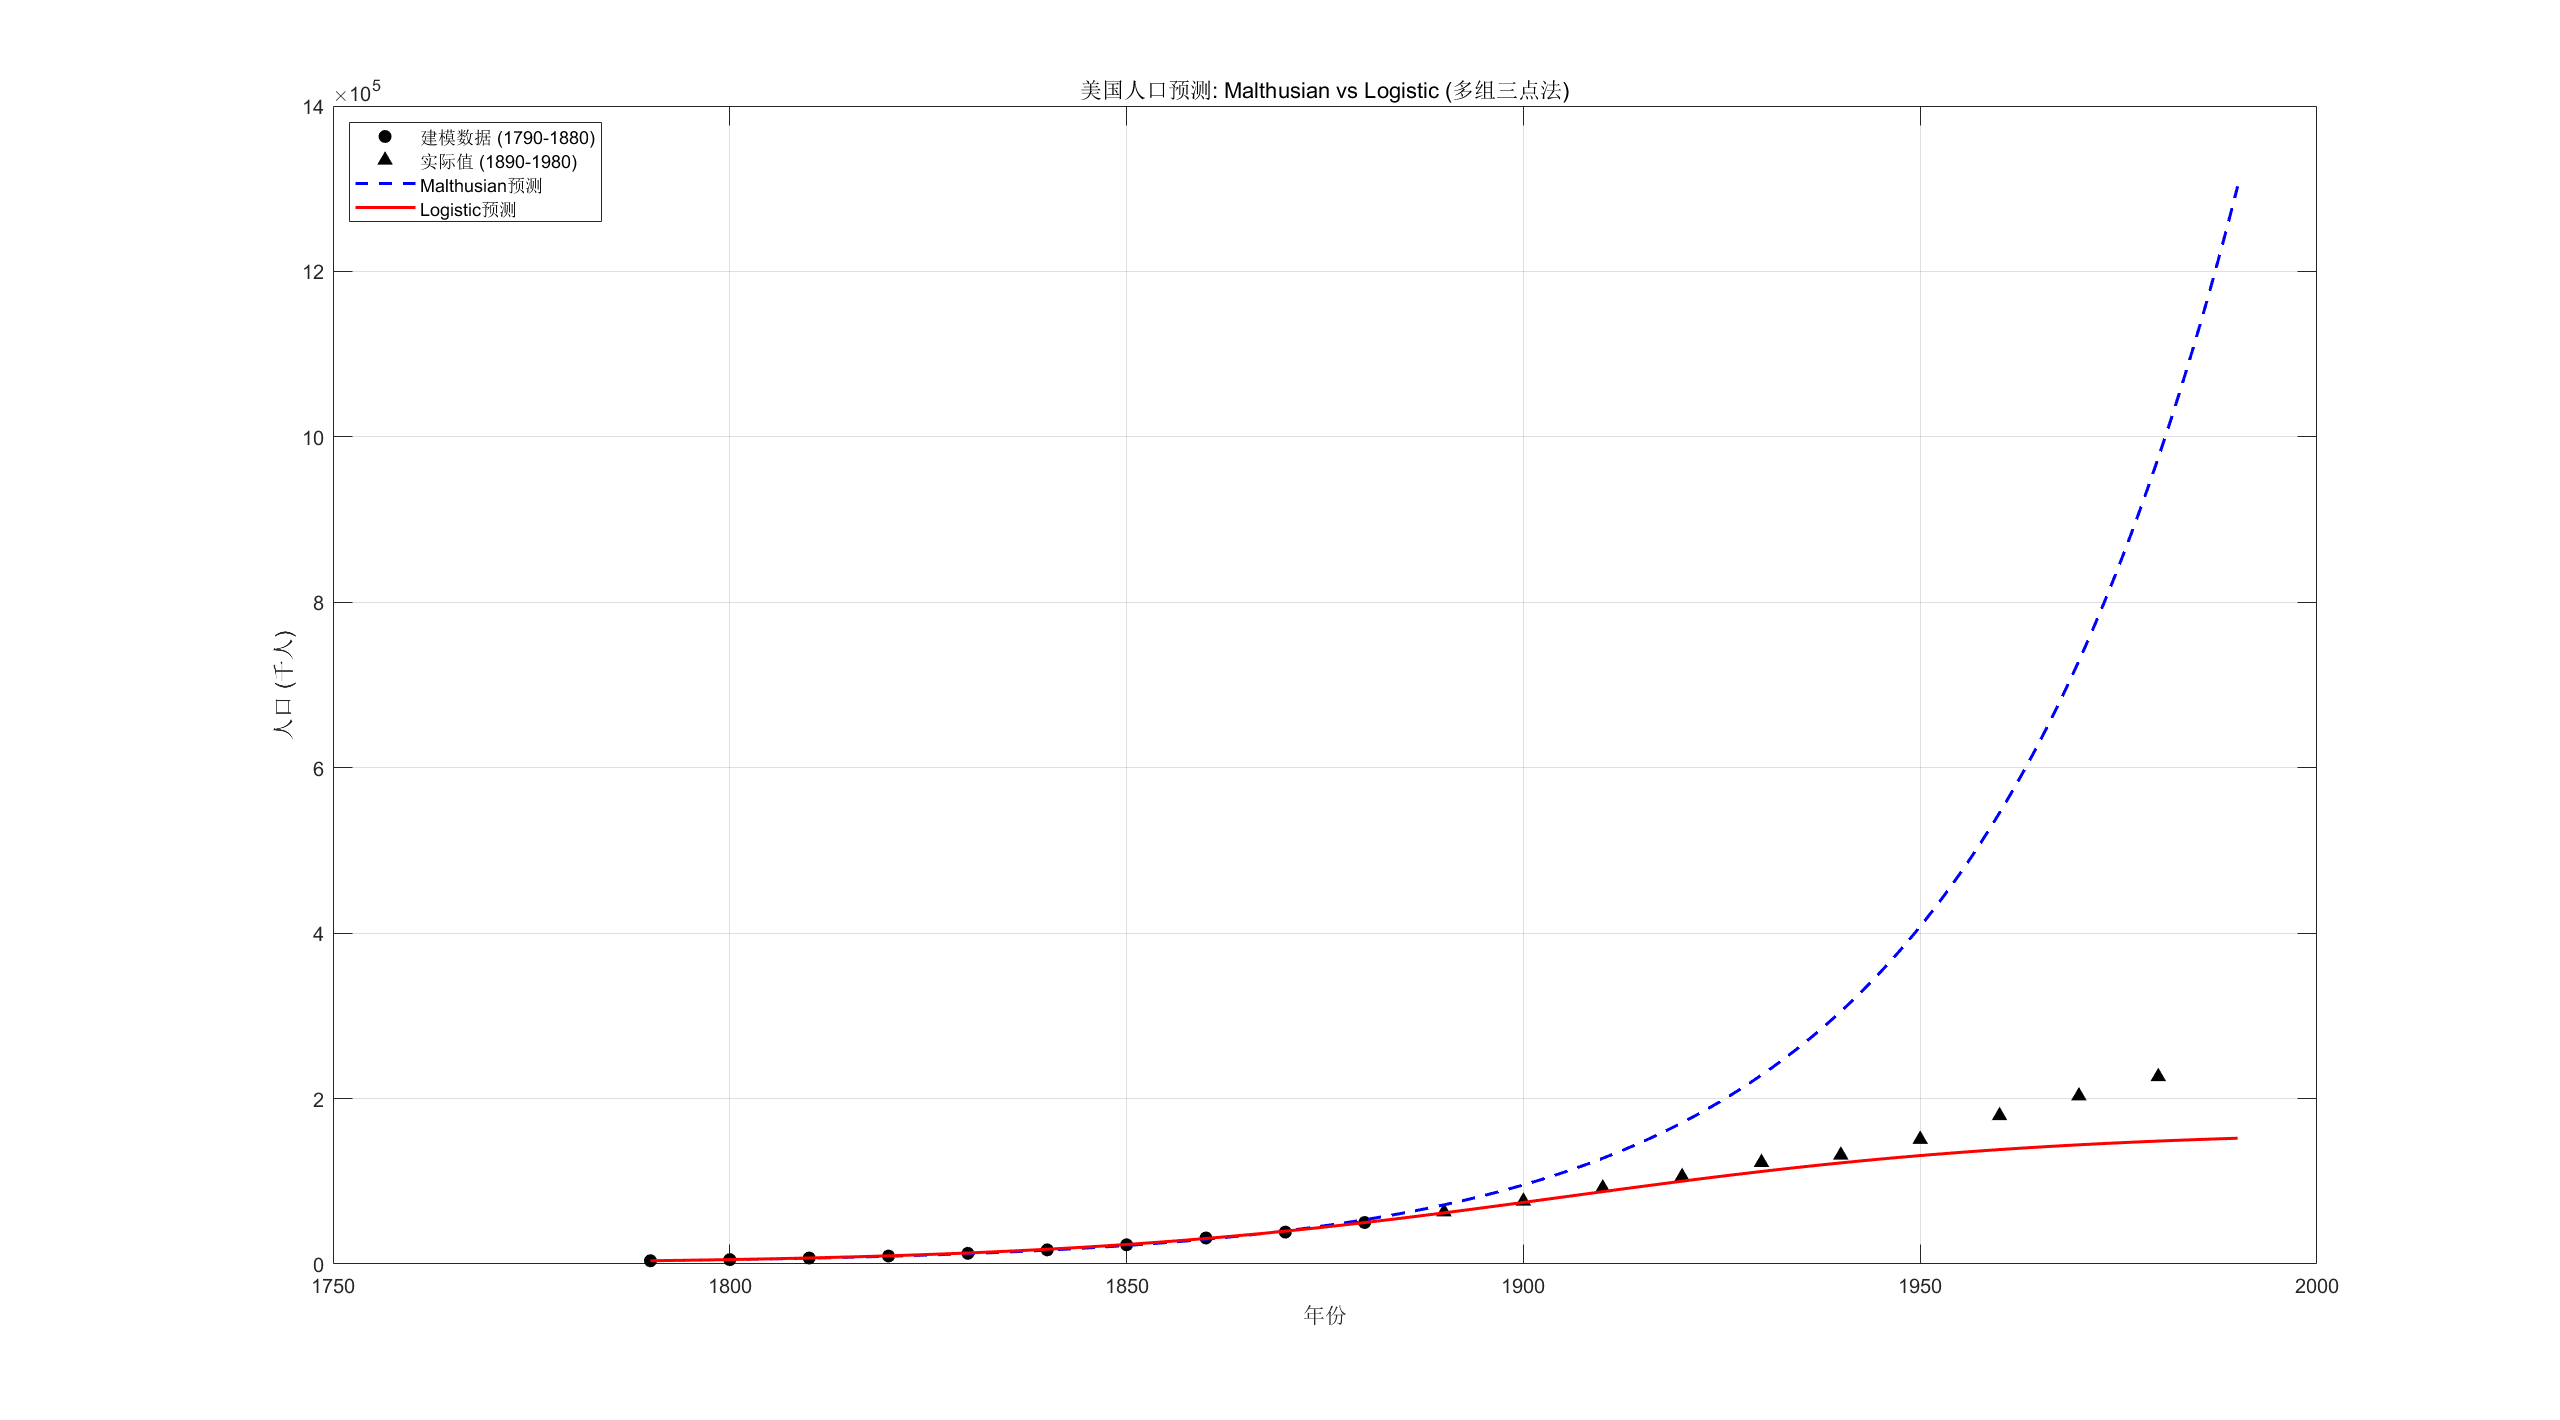
\includegraphics[width=\textwidth]{figure/HW4figure/MvsL.png}
\caption{Malthusian模型与Logistic模型预测对比}
\label{fig:mvsL}
\end{figure}

\section{模型比较}
为从多角度评价两模型的优劣，本节采用以下指标进行定量比较。

\subsection{拟合优度指标}
类似式(\ref{eq:rss})，定义预测残差平方和
\[
\text{RSS} = \sum_{i=1}^{10} (N_i^{\text{pred}} - N_i^{\text{true}})^2
\]
RSS越小表示拟合越好。为消除量纲影响，引入归一化指标
\[
\text{WRSS}=\sqrt{\frac{\text{RSS}}{\text{SSM}}}
\]
其中
$$
\text{SSM} = \sum_{i=1}^{10} (N_i^{\text{true}} - \bar{N}^{\text{true}})^2
$$

该值越小，模型拟合越好。
\subsection{模型选择准则 AIC}
为平衡拟合优度与模型复杂度，采用Akaike信息准则：
\[
\text{AIC} = n\ln\left(\frac{\text{RSS}}{n}\right) + 2p
\]
其中 $n=10$ 为样本数，$p$ 为模型参数个数。AIC越小，模型越优。

\subsection{比较结果}
两模型的定量比较结果如表\ref{tab:model_compare}所示。

\begin{table}[htbp]
\centering
\caption{两模型的定量比较}
\label{tab:model_compare}
\begin{tabular}{ccccc}
\toprule
模型 & 参数个数 $p$ & RSS & WRSS & AIC \\
\midrule
Malthusian & 1 & $1.08\times10^{12}$ & 6.36 & 27.41 \\
Logistic   & 2 & $1.17\times10^{10}$ & 0.66 & 24.88 \\
\bottomrule
\end{tabular}
\end{table}

由表可见：
\begin{itemize}
    \item Logistic模型的RSS比Malthusian模型小约两个数量级，归一化残差仅为0.66，远小于Malthusian的6.36。
    \item 尽管Logistic模型多一个参数，AIC仍比Malthusian模型低2.53，说明Logistic模型在增加一个参数的情况下大幅提升了拟合优度，综合表现更优。
    \item 从物理意义上，Malthusian假设资源无限与实际不符；Logistic引入容纳量概念，更符合"资源有限、环境承载力有限"的生物学直觉。
\end{itemize}

综上所述，Logistic模型在统计指标和物理解释两个层面均优于Malthusian模型。

\section{结论}
\begin{itemize}
    \item Malthusian模型假设增长率恒定、资源无限，长期预测必然出现指数爆炸。
    \item Logistic模型通过容纳量 $\bar{N}$ 引入密度制约，能描述增长饱和现象。
    \item 多组三点法取中位数配合线性回归，提高了参数估计的稳健性。
    \item 定量比较表明，Logistic模型在RSS、AIC等指标上均优于Malthusian模型。
\end{itemize}

\section*{附录：MATLAB代码}
\inputMATLAB{codes/HW4codes/main.m}
\textbf{代码说明：}
\begin{itemize}
    \item 多组三点法：遍历所有满足 $t_j-t_i = t_k-t_j$ 的三个点，用式(\ref{eq:threepoint})计算 $\bar{N}$，取中位数作为 $\hat{\bar{N}}$。
    \item 内禀增长率 $r$：在得到 $\hat{\bar{N}}$ 后，利用全部数据对 $\ln\frac{N}{\hat{\bar{N}}-N}$ 与 $t$ 作线性回归，得到更稳健的估计。
    \item 结果直接输出到命令窗口，可复制填入LaTeX表格。
\end{itemize}
